
%%%%%%%%%%%%%%%%%%%%%%%%%%%%%%%%%%%%%%%%%%%%%%%%%%%%%%%%

\chapter*{A - tRPC}
\addcontentsline{toc}{chapter}{\protect\numberline{}A - tRPC}

tRPC is a client-server framework for building scalable web applications. It allows developers to define procedures on the server side and call them from the client side using a strongly-typed API. \cite{trpc_offical} tRPC uses HTTP requests and responses to send and receive data between the client and server. It uses a three-tier architecture, where the client, server, and data flow are separated into these three layers. 

\bigbreak
\noindent
\textbf{Front-end} \\
Here, tRPC works by defining procedures that the client can call. These procedures are defined in a schema file, which describes the input and output types of each procedure. The client then uses a generated API to call these procedures.

\bigbreak
\noindent
\textbf{Middleware} \\
The middleware part of tRPC refers to the code that sits between the frontend and the backend. tRPC provides an Express middleware that intercepts requests and responses and can perform various operations such as authentication, logging, error handling, rate limiting, and caching. The middleware is designed to be modular, so multiple middlewares can be chained together to form a pipeline. 

\bigbreak
\noindent
\textbf{Back-end} \\
The back-end of tRPC is the actual server that receives and processes the requests from the frontend. It typically consists of a collection of microservices or functions that perform specific tasks and return the necessary data to the frontend.  

\bigbreak
\noindent
tRPC is designed to be flexible and can be used with any full-stack technology. It also includes built-in support for TypeScript and GraphQL. There's also support for subscriptions via Websockets. \cite{trpc_subscriptions}

% For included tables and figures renew the numbering such that they are numbered by the appendix they are attached to and not to the conclusion chapter
\renewcommand{\thefigure}{A.\arabic{figure}}
\setcounter{figure}{0}
\renewcommand{\thetable}{A.\arabic{table}}
\setcounter{table}{0}

\newpage
\section*{\large{A1 - tRPC data flow}}
\vspace*{1cm}

\begin{figure}[!ht]
   \begin{minipage}{1\textwidth}
     \centering
     \includesvg[width=.95\textwidth]{Figures/appendix/trpc-data-flows-edit-min.svg}
     \caption[Data flow in tRPC]{Figure showing the data flow in tRPC \cite{tRPC_dataflow_Ehrlich}
     }
     \label{trpc:figure}
   \end{minipage}\hfill
\end{figure}


%%%%%%%%%%%%%%%%%%%%%%%%%%%%%%%%%%%%%%%%%%%%%%%%%%%%%%%%

\newpage
\chapter*{B - Project description}
\label{chap:project-description}
\addcontentsline{toc}{chapter}{\protect\numberline{}B - Project description} 

This appendix includes the original project description, as presented in \autoref{requirements:description}, which we received during the application process for various Bachelor projects. Additionally, it contains the revised project requirements, depicted in \autoref{requirements:requirements}, which were developed following our first meeting with FiiZK where we clarified the goals. 


% For included tables and figures renew the numbering such that they are numbered by the appendix they are attached to and not to the conclusion chapter
\renewcommand{\thefigure}{B.\arabic{figure}}
\setcounter{figure}{0}
\renewcommand{\thetable}{B.\arabic{table}}
\setcounter{table}{0}

\newpage
\section*{\large{B1 - Project description}}
\vspace*{1cm}

\begin{figure}[!ht]
    \begin{minipage}{1\textwidth}
      \centering
      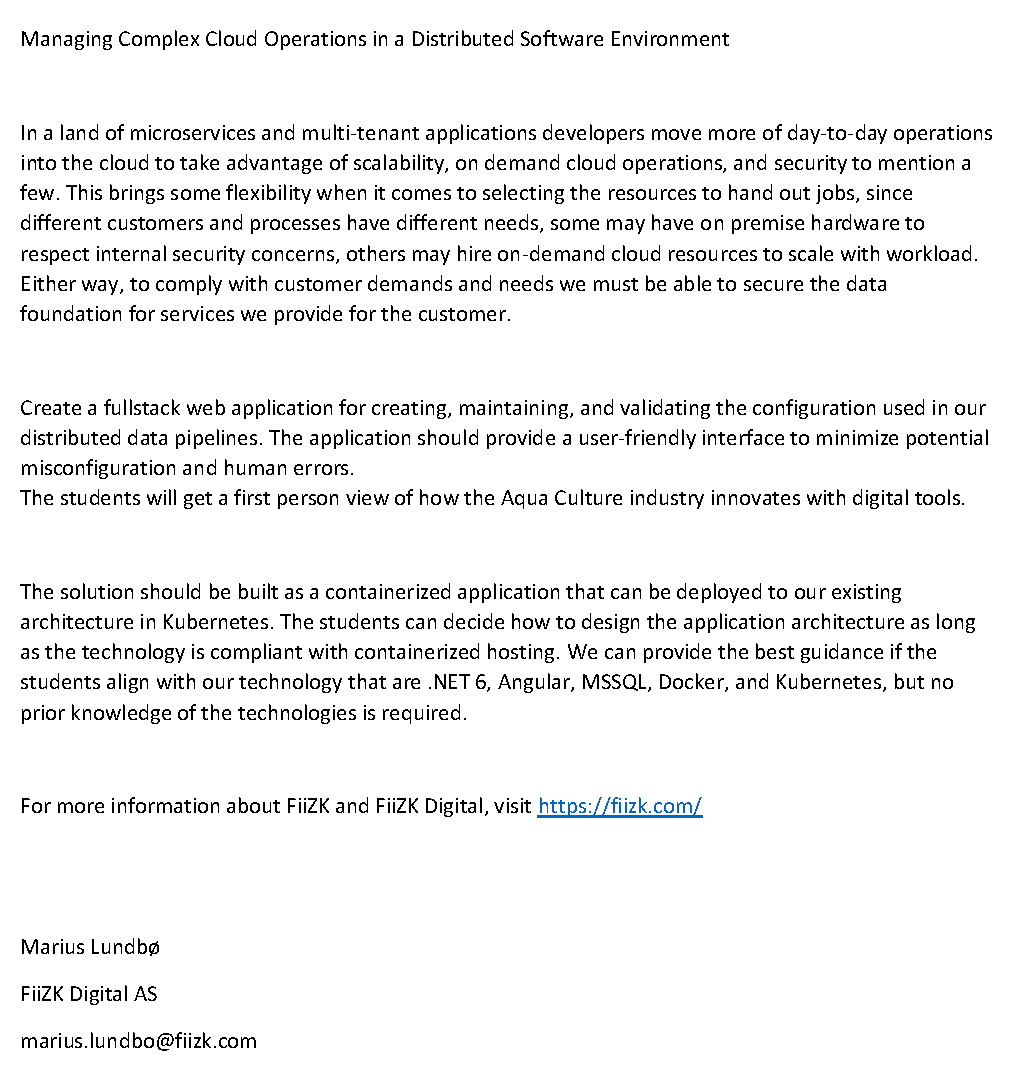
\includegraphics[width=.95\textwidth]{Figures/appendix/project-description.pdf}
     \caption[Original project description]{The original project description}
     \label{requirements:description}
    \end{minipage}\hfill
\end{figure}

\newpage
\section*{\large{B2 - Project requirements}}
\vspace*{1cm}

\begin{figure}[!ht]
\begin{minipage}{1\textwidth}
    \centering
        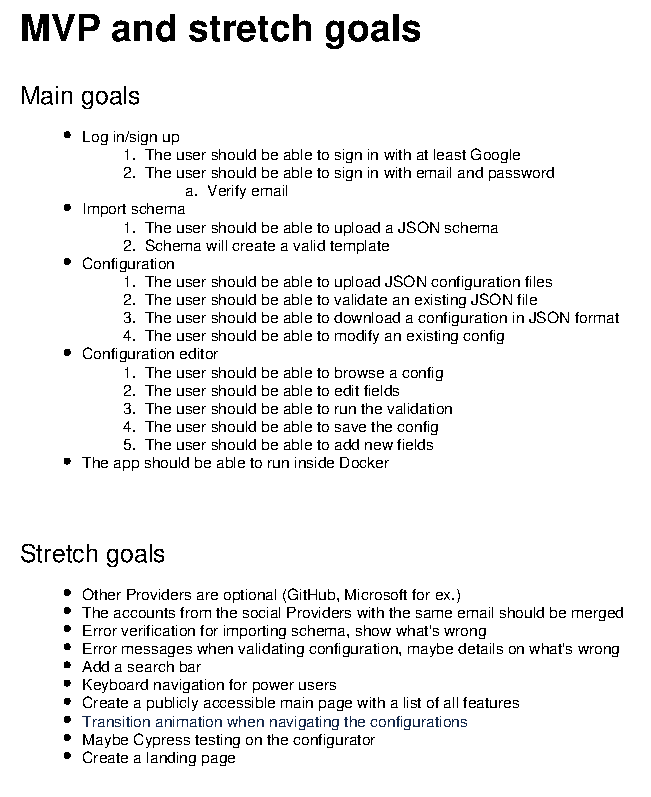
\includegraphics[width=.9\textwidth]{Figures/appendix/MVP and stretch goals.pdf}
        \caption[MVP and stretch goals]{The MVP and stretch goals}
        \label{requirements:requirements}
    \end{minipage}\hfill
\end{figure}

%%%%%%%%%%%%%%%%%%%%%%%%%%%%%%%%%%%%%%%%%%%%%%%%%%%%%%%%

\chapter*{C - Wireframes}
\addcontentsline{toc}{chapter}{\protect\numberline{}C - Wireframes}

These wireframes are a visual representations of the user interface design for our web application. They show the layout of each page, including the placement of buttons, forms, and other interactive elements.

% For included tables and figures renew the numbering such that they are numbered by the appendix they are attached to and not to the conclusion chapter
\renewcommand{\thefigure}{C.\arabic{figure}}
\setcounter{figure}{0}
\renewcommand{\thetable}{C.\arabic{table}}
\setcounter{table}{0}

\newpage
\section*{\large{C1 - Wireframes of the web application}}\label{wireframes:header}
\vspace*{1cm}

\begin{figure}[!ht]
    \begin{minipage}{1\textwidth}
         \centering
      \includegraphics[width=1\textwidth,page=6]{Figures/appendix/Wireframes.pdf}
     \caption[Sign in page wireframes]{A figure showing the sign in page}\label{wireframes:signin}
    \end{minipage}\hfill
\end{figure}

\vspace{1cm}

\begin{figure}[!ht]
    \begin{minipage}{1\textwidth}
         \centering
      \includegraphics[width=1\textwidth,page=14]{Figures/appendix/Wireframes.pdf}
     \caption[Account page wireframes]{A figure showing account page}\label{wireframes:account}
    \end{minipage}\hfill
\end{figure}


\begin{figure}[!ht]
    \begin{minipage}{1\textwidth}
         \centering
      \includegraphics[width=1\textwidth,page=7]{Figures/appendix/Wireframes.pdf}
     \caption[Templates page wireframes]{A figure showing the templates page}\label{wireframes:homescreen}
    \end{minipage}\hfill
\end{figure}

\vspace{1cm}

\begin{figure}[!ht]
    \begin{minipage}{1\textwidth}
         \centering
      \includegraphics[width=1\textwidth,page=8]{Figures/appendix/Wireframes.pdf}
     \caption[Configurations page wireframes]{A figure showing the configurations for a specific template}\label{wireframes:template}
    \end{minipage}\hfill
\end{figure}



\begin{figure}[!ht]
    \begin{minipage}{1\textwidth}
         \centering
      \includegraphics[width=1\textwidth,page=9]{Figures/appendix/Wireframes.pdf}
     \caption[Configuration browser wireframes]{A figure showing the configuration browser}
     \label{wireframes:configurationbrowser}
    \end{minipage}\hfill
\end{figure}

\vspace{1cm}

\begin{figure}[!ht]
    \begin{minipage}{1\textwidth}
         \centering
      \includegraphics[width=1\textwidth,page=24]{Figures/appendix/Wireframes.pdf}
     \caption[Error message wireframes]{A figure displaying the error messages}\label{wireframes:errormessages}
    \end{minipage}\hfill
\end{figure}

\clearpage
%%%%%%%%%%%%%%%%%%%%%%%%%%%%%%%%%%%%%%%%%%%%%%%%%%%%%%%%

\chapter*{D - Project manual}
\addcontentsline{toc}{chapter}{\protect\numberline{}D - Project manual}

Please refer to the separate attachment for additional information. \\

\iffalse

\bigbreak

\noindent
Oblig 2 Prosessdokumentasjon (Prosjekthåndbok)
\begin{itemize}
    \item Sprint reports: sprint reviews, sprint retrospectives
    \item Statusrapporter (ukentlig)
    \item Timelister (ukentlig)
    \item Møteinnkallinger og møtereferat
    \item Refleksjonsnotat (individuelle)
\end{itemize}
Innlevering: Inspera. Frist 22. Mai. 

\fi

%%%%%%%%%%%%%%%%%%%%%%%%%%%%%%%%%%%%%%%%%%%%%%%%%%%%%%%%

\chapter*{E - System Documentation}
\label{chap:system-documentation}
\addcontentsline{toc}{chapter}{\protect\numberline{}E - System Documentation}

% For included tables and figures renew the numbering such that they are numbered by the appendix they are attached to and not to the conclusion chapter
\renewcommand{\thefigure}{E.\arabic{figure}}
\setcounter{figure}{0}
\renewcommand{\thetable}{E.\arabic{table}}
\setcounter{table}{0}


% Change the numbering style for this section
\renewcommand{\thesection}{E.\arabic{section}}
\renewcommand{\thesubsection}{\arabic{subsection}}


This appendix provides detailed information about the project’s structure and code architecture. It includes an overview of the project’s organization and a description of how the code is designed and implemented.

\vspace{1.5cm}

% Start collection chapters for the local appendix contents
\startcontents[chapters]

\textbf{\Large Contents}
\vspace{0.5cm}
\printcontents[chapters]{}{1}{}

\newpage

% Shuts up the warning for sections levels, use with caution
\pdfbookmark[1]{Dummy}{dummy}

% Create a 'shadow' section, needed so that other subsections work
\section*{}

\iffalse
\subsubsection{Frontend}
The frontend was designed to provide a user-friendly interface for managing JSON configurations. It utilizes frontend technologies such as Next.js, NextAuth, and ChakraUI to create a visually appealing and responsive web application that is easy to use and navigate. The frontend was also integrated with the backend APIs using tRPC to ensure seamless communication between the frontend and backend components.
\fi

\subsection{Architecture}
The architecture of our full-stack web application consists of three main components: the frontend, backend, and database. These components work together to create a secure, scalable, and reliable system for managing configurations. In this section, we will provide an overview of the key features of each component and how they interact with one another.

\subsubsection{Frontend}
The frontend of our application was built using the Next.js framework and the ChakraUI component library. Next.js is a framework for building server-rendered React applications, and ChakraUI provides a set of pre-built React components that we used to create a customizable, accessible, and performant interface. \\

\noindent
To integrate the frontend with the backend, we used tRPC, a TypeScript-based Remote Procedure Call (RPC) framework. tRPC provided us with a set of React Query hooks for querying and mutating data, as well as middleware for validating authorization for protected endpoints. We also utilized React Query's caching system to automatically refresh data based on various conditions. \\

\noindent
Authentication in the frontend is handled using the NextAuth library, which provides a set of utilities for handling authentication actions such as sign ins and sign outs with different providers, account linking, and more.

\subsubsection{Backend} 
The backend of our application was designed to provide seamless development, security, stability, and scalability. It uses Next.js' built-in API Routes, tRPC, Prisma, and AJV. \\

\noindent
The RESTful API is built using tRPC, which allows us to create endpoints using procedures that define the route, input, and output of each endpoint. tRPC middleware is used to validate authorization for protected endpoints. Prisma is used to interact with the database, which is a PostgreSQL database.\\

\noindent
Authentication in the backend is integrated with Prisma using a Prisma adapter for NextAuth, which allows us to store authorization data for each user, such as session data, information about different providers the user has authenticated with, scopes, and refresh tokens. tRPC can directly access this data to authenticate the user for protected endpoints. \\

\noindent
AJV, a JSON schema validator, is used to validate all JSON configurations and schemas. It is contained within the validation tRPC endpoint. \\

\noindent
Overall, the architecture of our application provides a reliable and scalable solution for managing configurations. The frontend and backend components work together seamlessly to provide a user-friendly interface and a secure and efficient backend for managing data.


\begin{figure}[!ht]
    \begin{minipage}{1\textwidth}
    \centering
     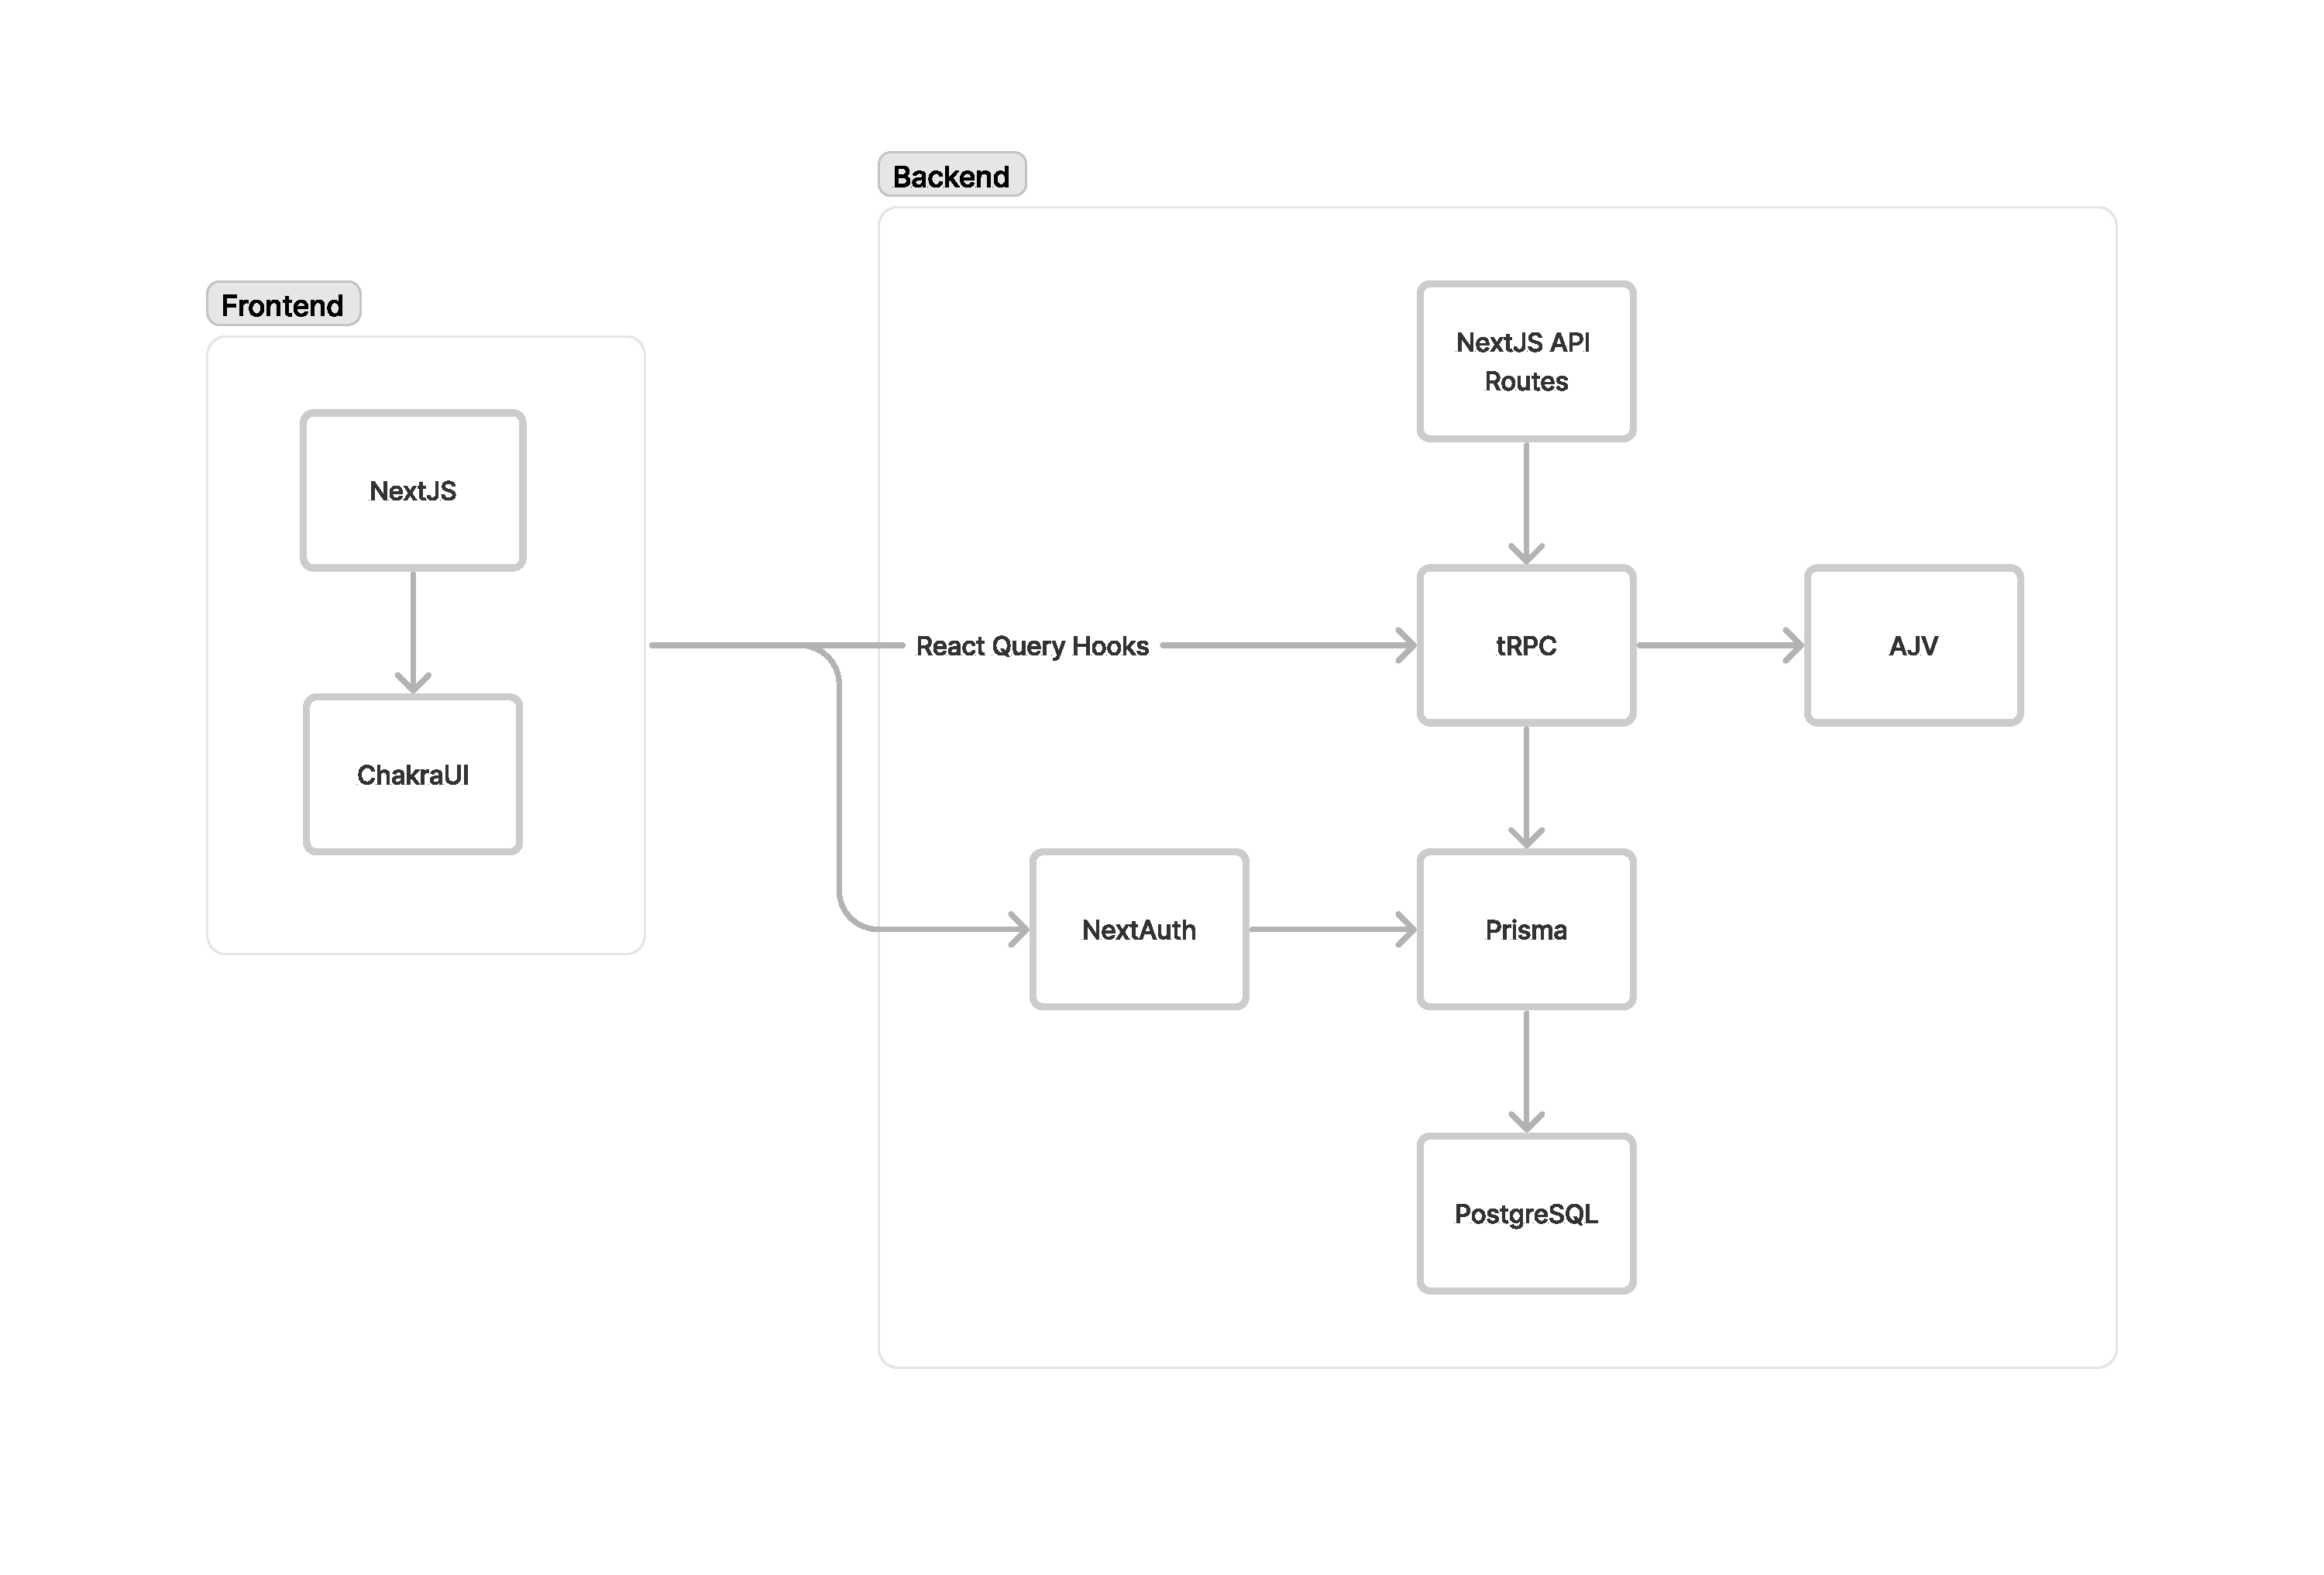
\includegraphics[width=0.9\textwidth]{Figures/appendix/architecture-overview-new.pdf}
     \caption[Overview of the software architecture]{A figure showing an overview of the software architecture}
     \label{architecture:overview}
    \end{minipage}\hfill
\end{figure}

\newpage

\subsection{Requirements Documentation}

\subsubsection{Use-case diagram}

\begin{figure}[!ht]
  \begin{minipage}{1\textwidth}
    \centering
    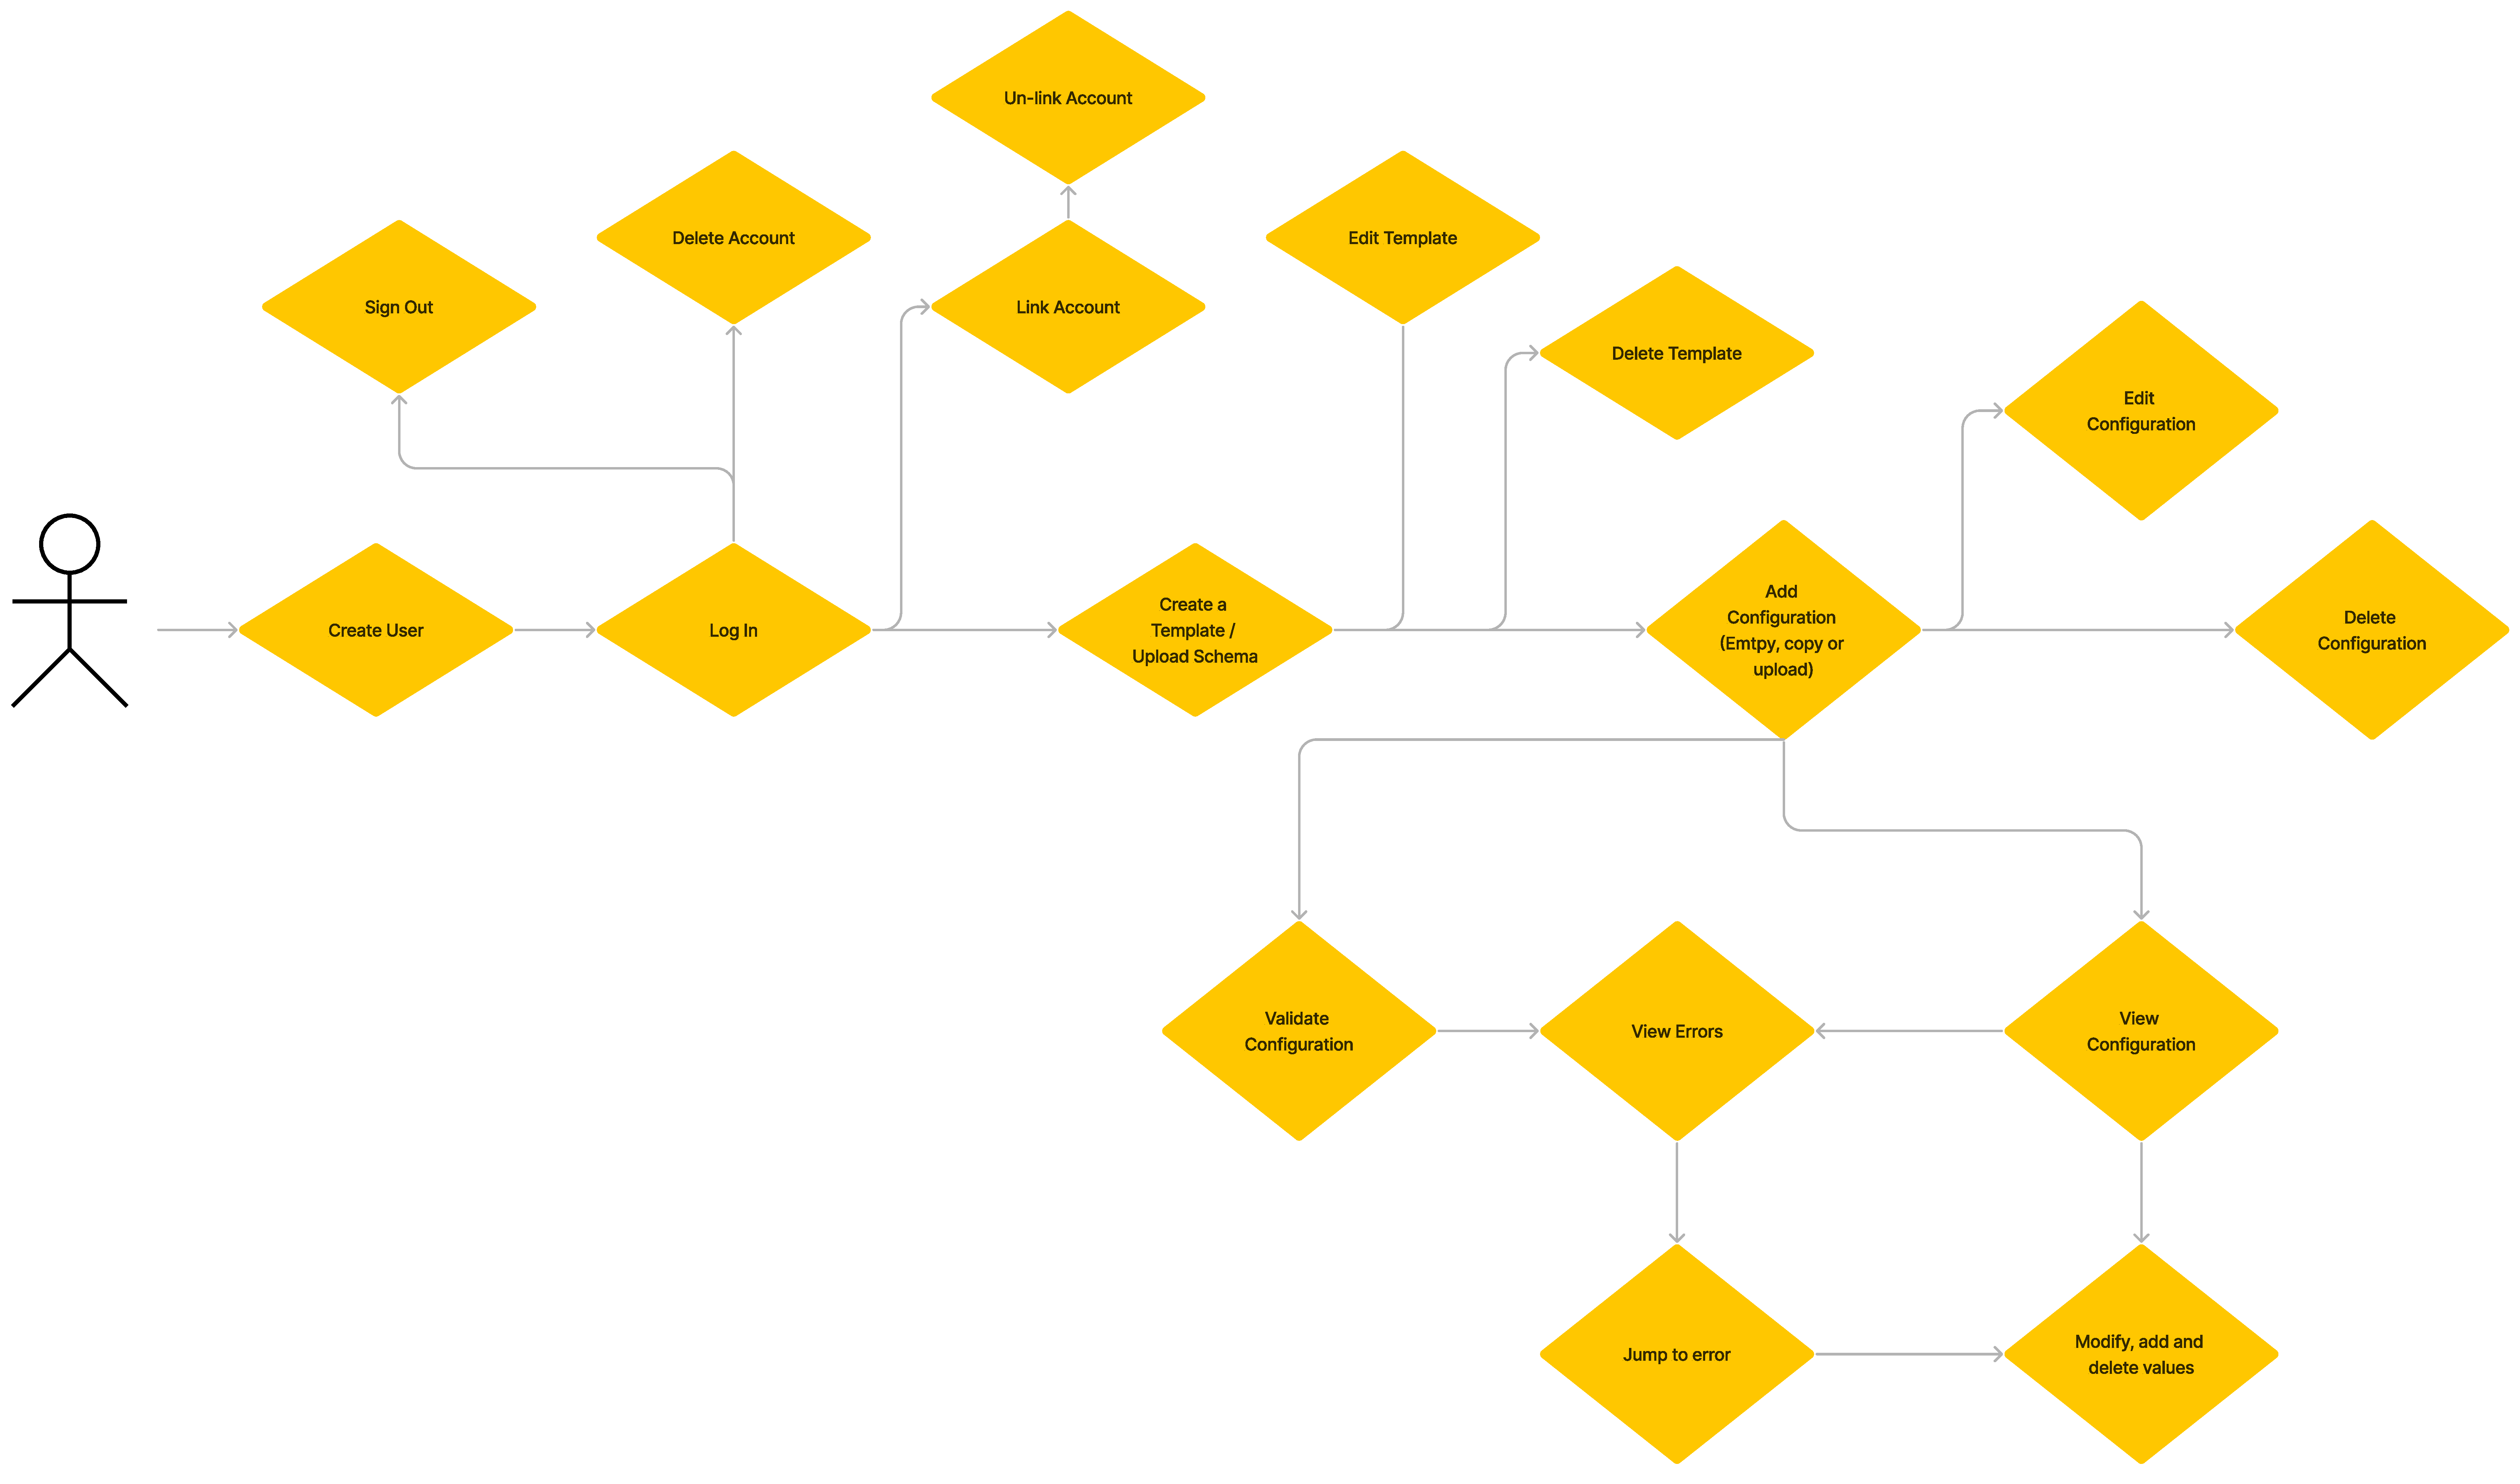
\includegraphics[width=1\textwidth]{Figures/appendix/UseCaseDiagram.pdf}
    \caption{Use-case Diagram}
    \label{usecasediagram}
  \end{minipage}\hfill
\end{figure}

\subsubsection{Project description}

Head to the \hyperref[chap:project-description]{Appendix B, Project description} to see the original task description and the MVP/stretch goals.

\newpage

\subsection{Project structure}

% - Talk about the folder structure and where the different parts of the app are

Next.js provides a comprehensive solution for developing and deploying web applications with features for both front-end and back-end. Consequently, we have organized our code in the following manner. For the front-end, Next.js utilizes a file-system-based router, where each file in the "pages" folder represents a unique page of the application. The "components" folder contains reusable React components that can be imported into different pages, while the "public" folder stores static assets, such as images, fonts, or other files, that can be served by the application. \\

\noindent
For the back-end, we have created a "server" folder to house server-side code that interacts with databases or external APIs, including our tRPC code. Additionally, we have other folders, such as "theme", "utils", or "types", that contain various components, utilities, and type definitions utilized throughout the project. \\

\noindent
For a better overview of the directory tree, see the 
\autoref{dirtree:figure}

\newpage
\vspace*{2cm}

% Generated using the tree command in Windows
\begin{figure}
    \dirtree{%
    .1 root.
    .2 prisma.
    .2 public.
    .3 assets.
    .4 animations.
    .2 src.
    .3 components.
    .4 avatars.
    .4 buttons.
    .4 cards.
    .4 configuration-browser.
    .5 hooks.
    .5 utils.
    .4 dialogs.
    .4 inputs.
    .4 layouts.
    .3 env.
    .3 pages.
    .4 api.
    .5 auth.
    .5 trpc.
    .4 auth.
    .4 configurations.
    .4 profile.
    .4 templates.
    .3 server.
    .4 api.
    .5 routers.
    .3 theme.
    .3 types.
    .3 utils.
    .4 validator.
    }
    \caption{The directory tree of the project}
    \label{dirtree:figure}
\end{figure}

\newpage

\subsection{Functional programming}

We employed functional programming paradigms in our project extensively. We utilized TypeScript, a super-set of the JavaScript language which provides support for both object-oriented and functional programming paradigms. Additionally, the Next.js framework, built on top of React, allows for the flexibility of choosing between functional and object-oriented programming paradigms with it's functional components and class components. The theory behind these two paradigms can be found in \autoref{sec:OO-programming} and \autoref{sec:functional-programming}. \\

\noindent
We opted to utilize the newer React functional components in our project, as they offer several key advantages. Functional components result in a more concise codebase that is easier to comprehend and maintain. This approach aligns with the functional programming principles of immutability and pure functions, enabling us to write cleaner and predictable code. \\

\noindent
One of the key benefits of functional components is the ability to utilize React hooks. Hooks allow us to manage state and side effects in a more declarative and composable manner, enhancing code modularity and reusability. By leveraging hooks, we were able to effectively handle complex functionalities such as authentication and data fetching, including caching and refetching via TanStack Query hooks. The theory behind hooks has been covered in \autoref{sec:hooks-theory} and more detailed info on TanStack Query can be found in \autoref{sec:tanStack_query}. \\

% \todo{What else did hooks allow us to do?}

\newpage

\subsection{Database}
\label{chap:database-schema}

The database for this project uses the Prisma ORM and is written as a Prisma schema. It is implemented using a PostgreSQL database. The schema itself is divided into several tables that represent the different entities in the system, including User, Account, Session, Template, Configuration, and VerificationToken. \\

\noindent
The User model is used to store user information such as their name, email, and image URL. This model also has relationships with other models such as Account, Session, Template, and Configuration. The Account model is used to link user accounts from various providers, such as Google and GitHub. The Session model is used to store session information for authenticated users. \\

\noindent
The Template model is used to store templates that can be used to validate configurations. The Configuration model is used to store user-generated configurations. This model includes a list of ConfigurationError entities that are associated with it and indicate any errors in the configuration. The VerificationToken model is used to store tokens that are generated when a user requests to verify their email address.

\noindent
The complete database schema can be seen in \autoref{database:schema}.

\newpage
\subsection{Database schema}
\vspace*{1cm}

\begin{figure}[!ht]
    \begin{minipage}{1\textwidth}
         \centering
      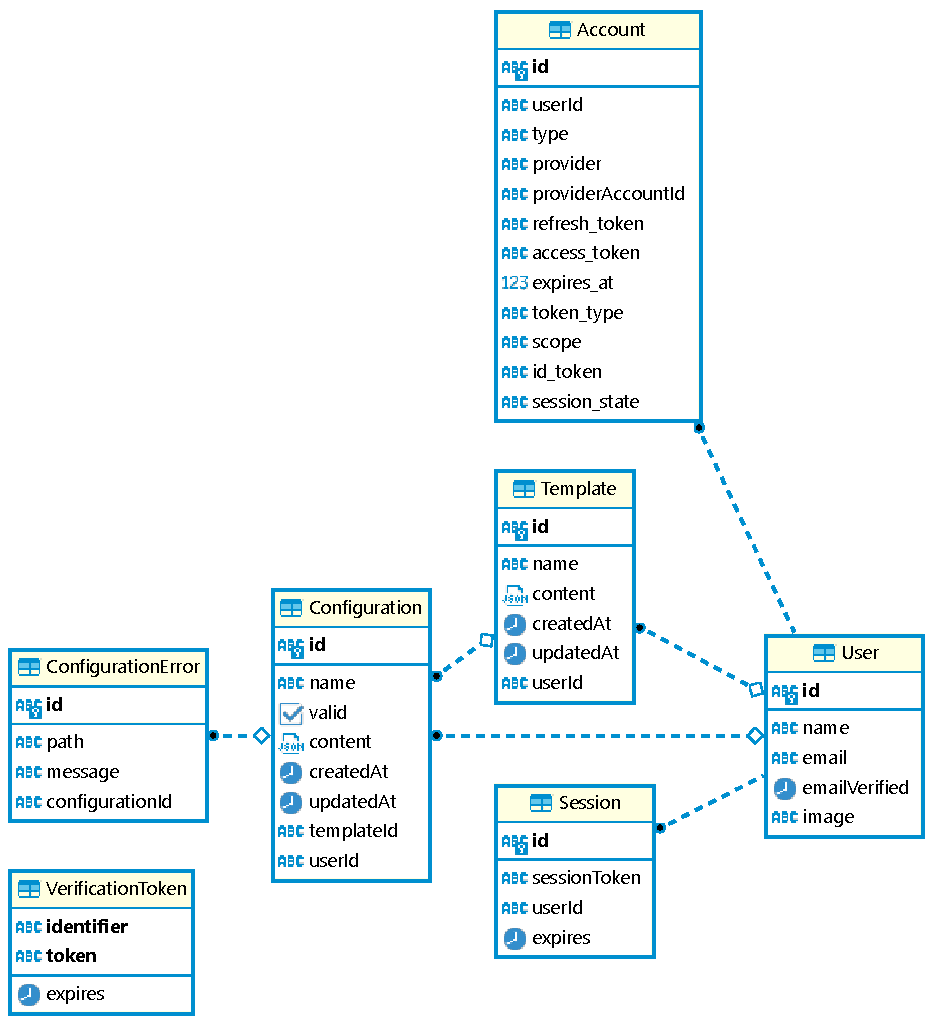
\includegraphics[width=.95\textwidth]{Figures/appendix/DB-schema.pdf}
     \caption[Database schema]{A figure showing the database schema}
     \label{database:schema}
    \end{minipage}\hfill
\end{figure}

\newpage

\subsection{Server endpoints}

This subsection describes the various tRPC endpoints available on the server for different functionalities such as configurations, user management, templates, and validation. These endpoints allow clients to perform CRUD operations on various data entities on the server.

\subsubsection{Configurations}

These are the tRPC server CRUD operations for the configurations. \\

\noindent
\textbf{getAll} \\
Retrieves all configurations for the authenticated user. It accepts an optional \textit{templateId} query parameter that filters the configurations based on the parameter if given. \\

\noindent
\textbf{get} \\
This method retrieves a single configuration by the \textit{id} and the authenticated user id. \\

\noindent
\textbf{add} \\
The add method creates a new configuration for the authenticated user. It accepts \textit{templateId}, \textit{name}, \textit{valid}, and \textit{content} inputs. The content input is validated against the JSON schema of the template associated with the configuration and the errors are generated if necessary. \\

\noindent
\textbf{delete} \\
Deletes a configuration by \textit{id} for the authenticated user. \\

\noindent
\textbf{clone} \\
Creates a new configuration by cloning an existing configuration by \textit{id} for the authenticated user. \\

\noindent
\textbf{download} \\
This method retrieves a configuration by \textit{id} for the authenticated user, encodes it as Base64, and then returns the configuration as a string. \\

\noindent
\textbf{update} \\
Updates an existing configuration by \textit{id} for the authenticated user. It accepts \textit{name} and \textit{content} inputs. The \textit{content} input is validated against the JSON schema of the template associated with the configuration and the errors are generated as needed. \\

\subsubsection{Me}

These endpoints are used for account data fetching and management. \\

\noindent
\textbf{get} \\
Retrieves the user information in a User object, including all associated accounts based on the user \textit{id} in the current session. \\

\noindent
\textbf{delete} \\
Deletes the user account based on the user \textit{id} in the current session. \\

\noindent
\textbf{unlink} \\
Removes the association between the user account and the specified third-party account provider based on the user \textit{id} and \textit{provider} name given as the input. \\

\subsubsection{Templates}

REST endpoints for managing the templates. \\

\noindent
\textbf{getAll} \\
Returns an array of all templates belonging to the currently authenticated user, along with the count of configurations associated with each template. \\

\noindent
\textbf{get} \\
Returns a specific template belonging to the currently authenticated user, identified by the provided \textit{id}. \\

\noindent
\textbf{add} \\
This endpoint creates a new template belonging to the currently authenticated user, with the provided \textit{name} and \textit{content} (if any). \\

\noindent
\textbf{delete} \\
Deletes a specific template belonging to the currently authenticated user, identified by the provided \textit{id}. \\

\noindent
\textbf{update} \\
The method updates a specific template belonging to the currently authenticated user, identified by the provided \textit{id}. The name and/or content of the template can be modified, and if the content is modified, the associated configurations are checked for validity using a validation function before being updated. \\

\subsubsection{Validate}

Endpoint used for validation. This is also the only public endpoint on the server meaning it can be accessed without authentication. \\

\noindent
\textbf{validate} \\
Validates a JSON configuration against a JSON schema and returns whether the configuration is valid and any errors encountered during validation. The configuration and schema are provided as strings in the input. Returns an object with a boolean value indicating whether the configuration is valid, and an array of error objects if any errors were encountered during validation. Each error object contains a path to the location of the error within the configuration and a message describing the error. \\

\subsection{Security}
% - Maybe worth a mention, not a focus for the project? \\
% - Endpoints are secure \\
% - We don't store any passwords, only tokens \\

We have implemented several security measures to safeguard our data and server endpoints against unauthorized access. \\

\noindent
In the context of tRPC, we have established both public and protected procedures. These procedures enable us to differentiate between endpoints that are accessible to the public and those that require authorization. For protected procedures, we employ a middleware method that receives the authentication session for each request, ensuring that only authenticated users can access our private endpoints. Additionally, this approach prevents users from querying data that does not belong to them by verifying the stored user authorization token. \\

\noindent
Authentication is handled through the implementation of the NextAuth library. By leveraging NextAuth, we are able to eliminate the need to store or encrypt user passwords in our database. Instead, we utilize secure tokens provided by authentication providers to manage user sessions and access control. This approach significantly reduces the risk of password leaks and mitigates other common security vulnerabilities.

\subsection{Deployment}
% - How it's deployed \\
% - Name ALL the libraries used in the project

We deployed our application to Vercel, a cloud platform for serverless deployment of web applications. Vercel was a great choice for our deployment needs as it provides seamless integration with Next.js and a continuous deployment feature which automatically deploys changes to the live site whenever changes are pushed to our GitHub repository. \\

\noindent
In addition to deploying to Vercel, we also used a free database instance on Render.com for our production database. \\

\subsubsection{Libraries}

Here's a list of libraries and frameworks we used throughout the project. 

\begin{itemize}
    \item \textbf{@chakra-ui/react}: A library for building accessible and responsive user interfaces with React.
    \item \textbf{@emotion/react}: A library for writing CSS styles with JavaScript.
    \item \textbf{@emotion/styled}: A library for creating styled React components using CSS-in-JS.
    \item \textbf{@next-auth/prisma-adapter}: An adapter for using Prisma with NextAuth.js.
    \item \textbf{@prisma/client}: An auto-generated and type-safe database client.
    \item \textbf{@tanstack/react-query}: A library for fetching, caching and updating asynchronous data in React.
    \item \textbf{@trpc/client}: A library for making type-safe API calls to a tRPC server.
    \item \textbf{@trpc/next}: A library for integrating tRPC with Next.js.
    \item \textbf{@trpc/react-query}: A library for integrating tRPC with React Query.
    \item \textbf{@trpc/server}: A library for creating a tRPC server.
    \item \textbf{ajv}: A JSON schema validator.
    \item \textbf{chakra-react-select}: A Chakra UI styled version of the react-select component.
    \item \textbf{eslint}: A pluggable and configurable linter tool for identifying and reporting on patterns in JavaScript and TypeScript.
    \item \textbf{eslint-config-next}: An ESLint configuration for Next.js.
    \item \textbf{framer-motion}: A library for animating React components.
    \item \textbf{javascript-time-ago}: A library for formatting relative time strings.
    \item \textbf{lodash-es}: A modern JavaScript utility library delivering modularity, performance and extras.
    \item \textbf{next}: A React-based framework for building server-rendered or statically-exported React applications.
    \item \textbf{next-auth}: An authentication library for Next.js applications.
    \item \textbf{nodemailer}: A module for sending emails from Node.js applications.
    \item \textbf{prettier}: An opinionated code formatter that supports multiple programming languages.
    \item \textbf{react}: A JavaScript library for building user interfaces.
    \item \textbf{react-dom}: The entry point of the DOM-related rendering paths in React applications.
    \item \textbf{react-icons}: A collection of popular icon packs to use in React projects.
    \item \textbf{react-json-view}: A component for displaying and editing JSON data in React applications.
    \item \textbf{react-lottie}: A component for rendering Lottie animations in React applications.
    \item \textbf{react-time-ago}: A component for formatting relative time strings in React applications.
    \item \textbf{seedrandom}: A seeded random number generator for JavaScript, used to generate colors from strings in our project.
    \item \textbf{superjson}: An enhanced version of JSON that supports more data types and allows custom serialization logic.
    \item \textbf{trpc-openapi}: A tool for generating OpenAPI documentation from a tRPC server definition.
    \item \textbf{typescript}: A typed superset of JavaScript that compiles to plain JavaScript.
    \item \textbf{use-file-picker}: A hook for opening file picker dialogs in React applications.
    \item \textbf{zod}: A TypeScript-first schema validation library. 
\end{itemize}


\subsection{Documentation of source code}

During the development of the project, we made sure to document the code appropriately. We used descriptive names for functions and variables to make the code more readable and understandable. For more complex or harder to understand pieces of code, we included comments using the // syntax to explain the logic behind them. Additionally, if we were inspired by or borrowed code from other sources, we included references in the comments. 

% Change the numbering style back to the default style
\renewcommand{\thesection}{\thechapter.\arabic{section}}
\renewcommand{\thesubsection}{\thesection.\arabic{subsection}}

% Stop collecting contents for the partial table of contents
\stopcontents[chapters]

%%%%%%%%%%%%%%%%%%%%%%%%%%%%%%%%%%%%%%%%%%%%%%%%%%%%%%%%

\newpage
\chapter*{F - Repository}
\addcontentsline{toc}{chapter}{\protect\numberline{}F - Repository} 

\renewcommand{\thefigure}{F.\arabic{figure}}
\setcounter{figure}{0}
\renewcommand{\thetable}{F.\arabic{table}}
\setcounter{table}{0}

The source code for our project can be found on GitHub at the following URL: \url{https://github.com/nilssen98/bachelor-project}. A .zip file containing the source code is also included as a separate attachment with this thesis.

%%%%%%%%%%%%%%%%%%%%%%%%%%%%%%%%%%%%%%%%%%%%%%%%%%%%%%%%

\iffalse

% Leftover from the template, not rendered 

\renewcommand{\thefigure}{X.\arabic{figure}}
\setcounter{figure}{0}
\renewcommand{\thetable}{X.\arabic{table}}
\setcounter{table}{0}

% Page without title but section title:
\newpage
\section*{\large{X2 - Some other random table}}
\vspace*{1cm}

\begin{table}[ht!]
\centering
    \begin{tabular}{ m{4cm} m{2.5cm} m{2.5cm} m{2.5cm} } 
    \toprule
    \toprule
    \textbf{Statistic} & \textbf{Three} & \textbf{Four}  \\
    \midrule
    Count   & 387317    & 283960    \\[1.3ex]
    Mean    & 130.66    & 134.18    \\[1.3ex]
    Std     & 248.09    & 230.32    \\[1.3ex]
    Q1      & 31.00     & 21.00     \\[1.3ex]
    Median  & 67.00     & 63.00     \\[1.3ex]
    Q3      & 142.00    & 159.00    \\[1.3ex]
    Min     & 0.00      & 0.00      \\[1.3ex]
    Max     & 14519.00  & 14253.00  \\[1.3ex]
    \bottomrule
    \bottomrule
    \end{tabular}
\caption[Statistics on something else]{Table of statistics on some other sidenote data.}
\end{table}



\newpage
\section*{\large{X3 - Some random figure}}
\vspace*{1cm}

\begin{figure}[H]
  \centering
  \subfloat[Data set sizes for data X.]
  {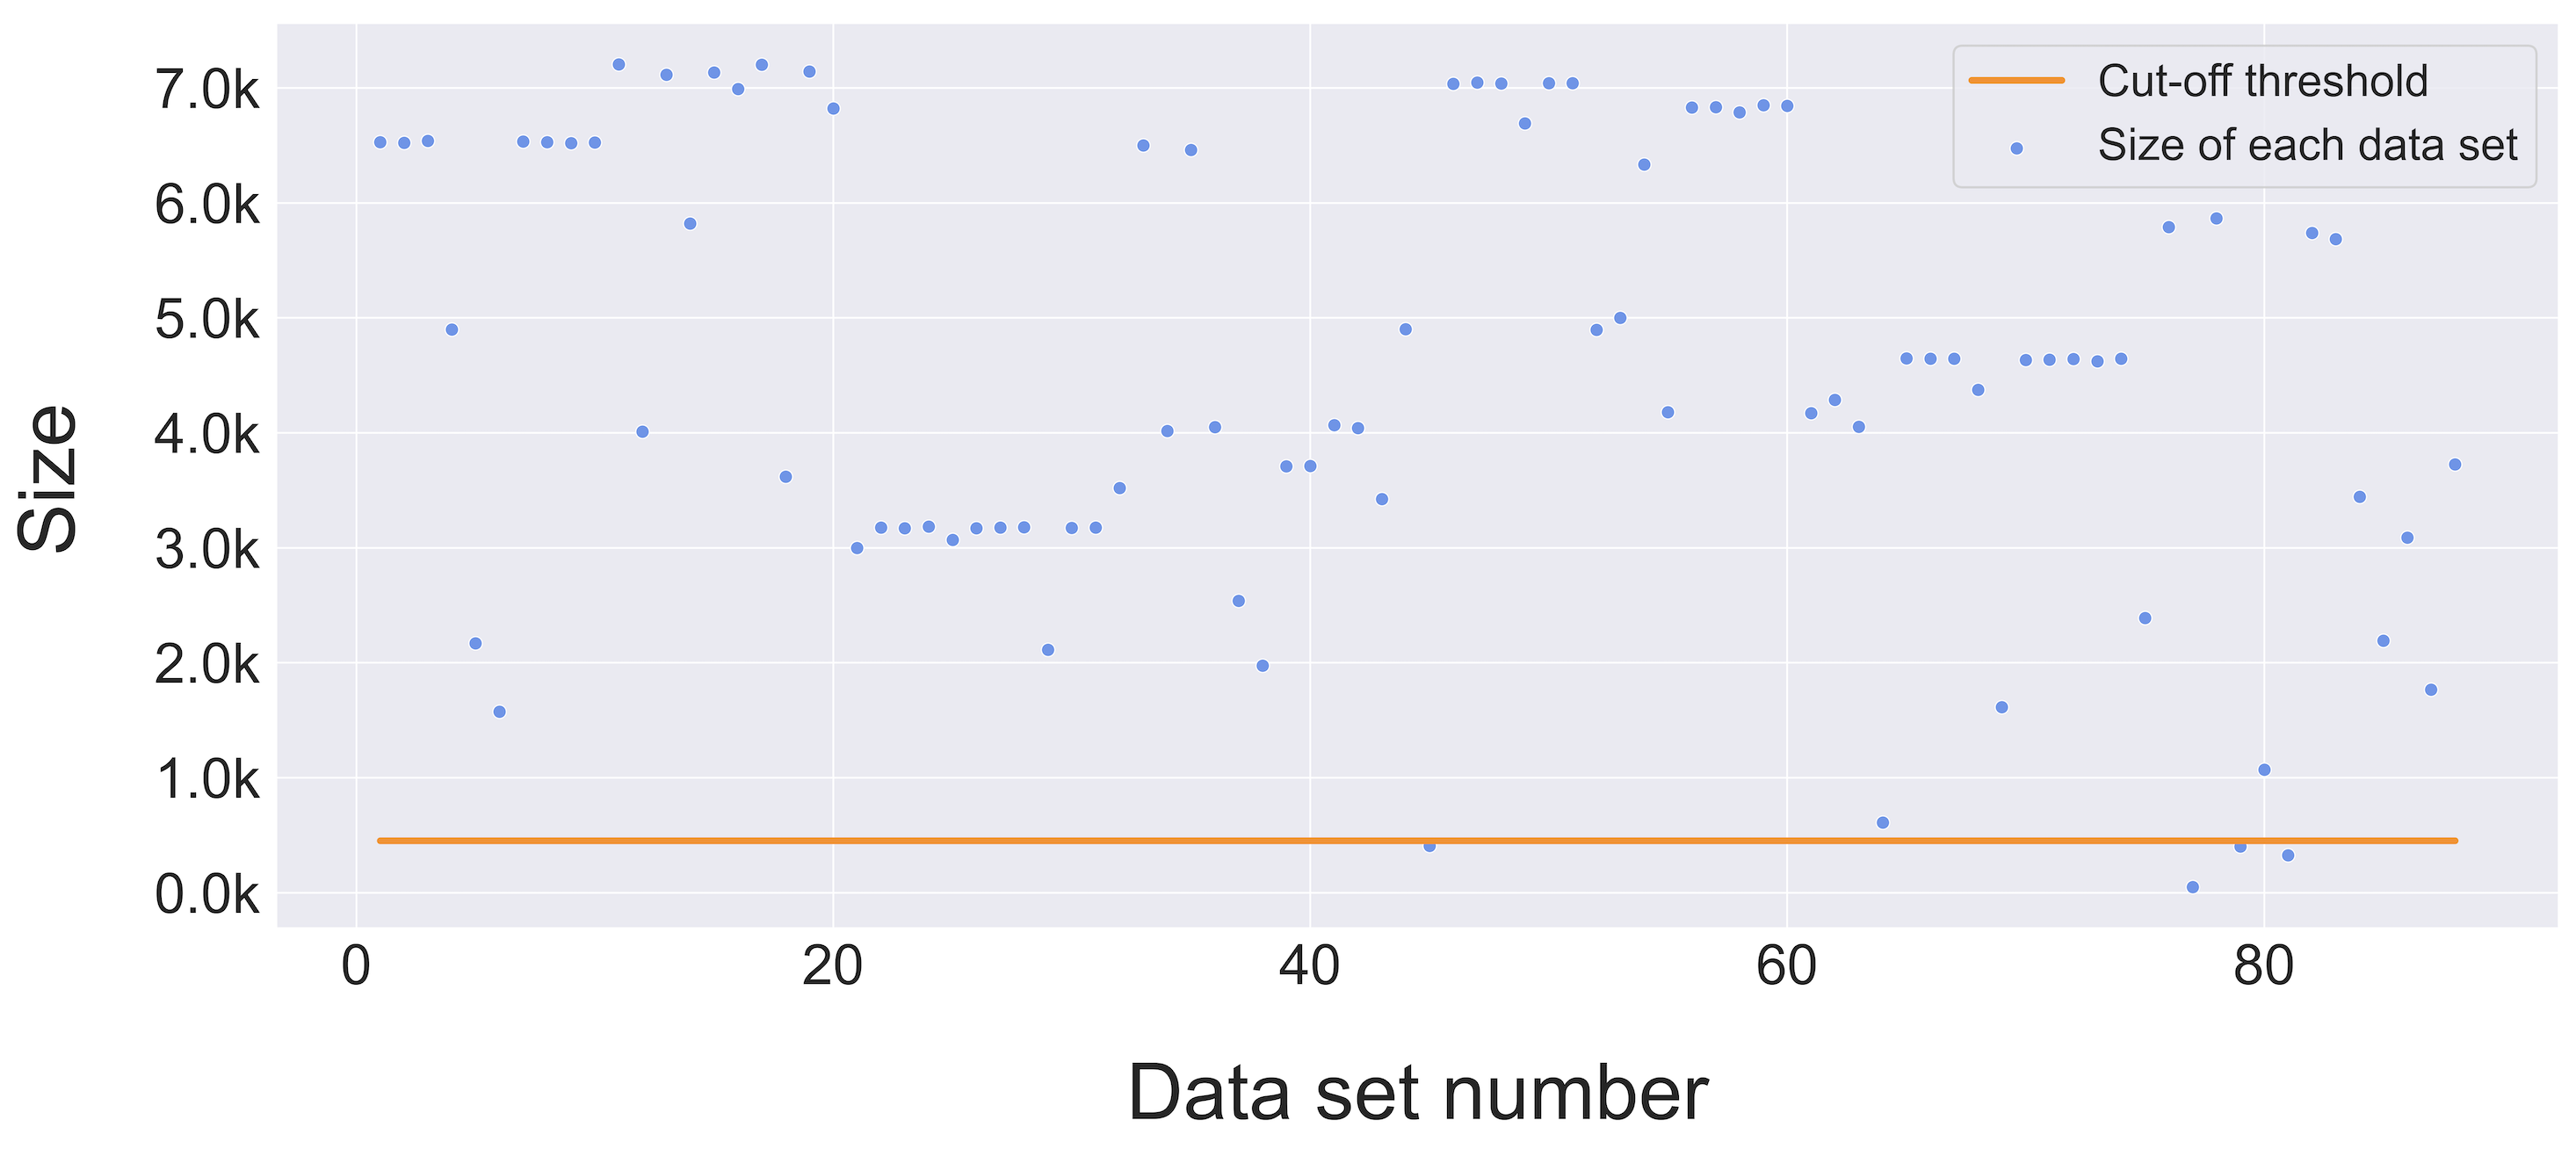
\includegraphics[width=1\textwidth]{Figures/dataset_X.png}}
  \hfill
  \subfloat[Data set sizes for data Y.]
  {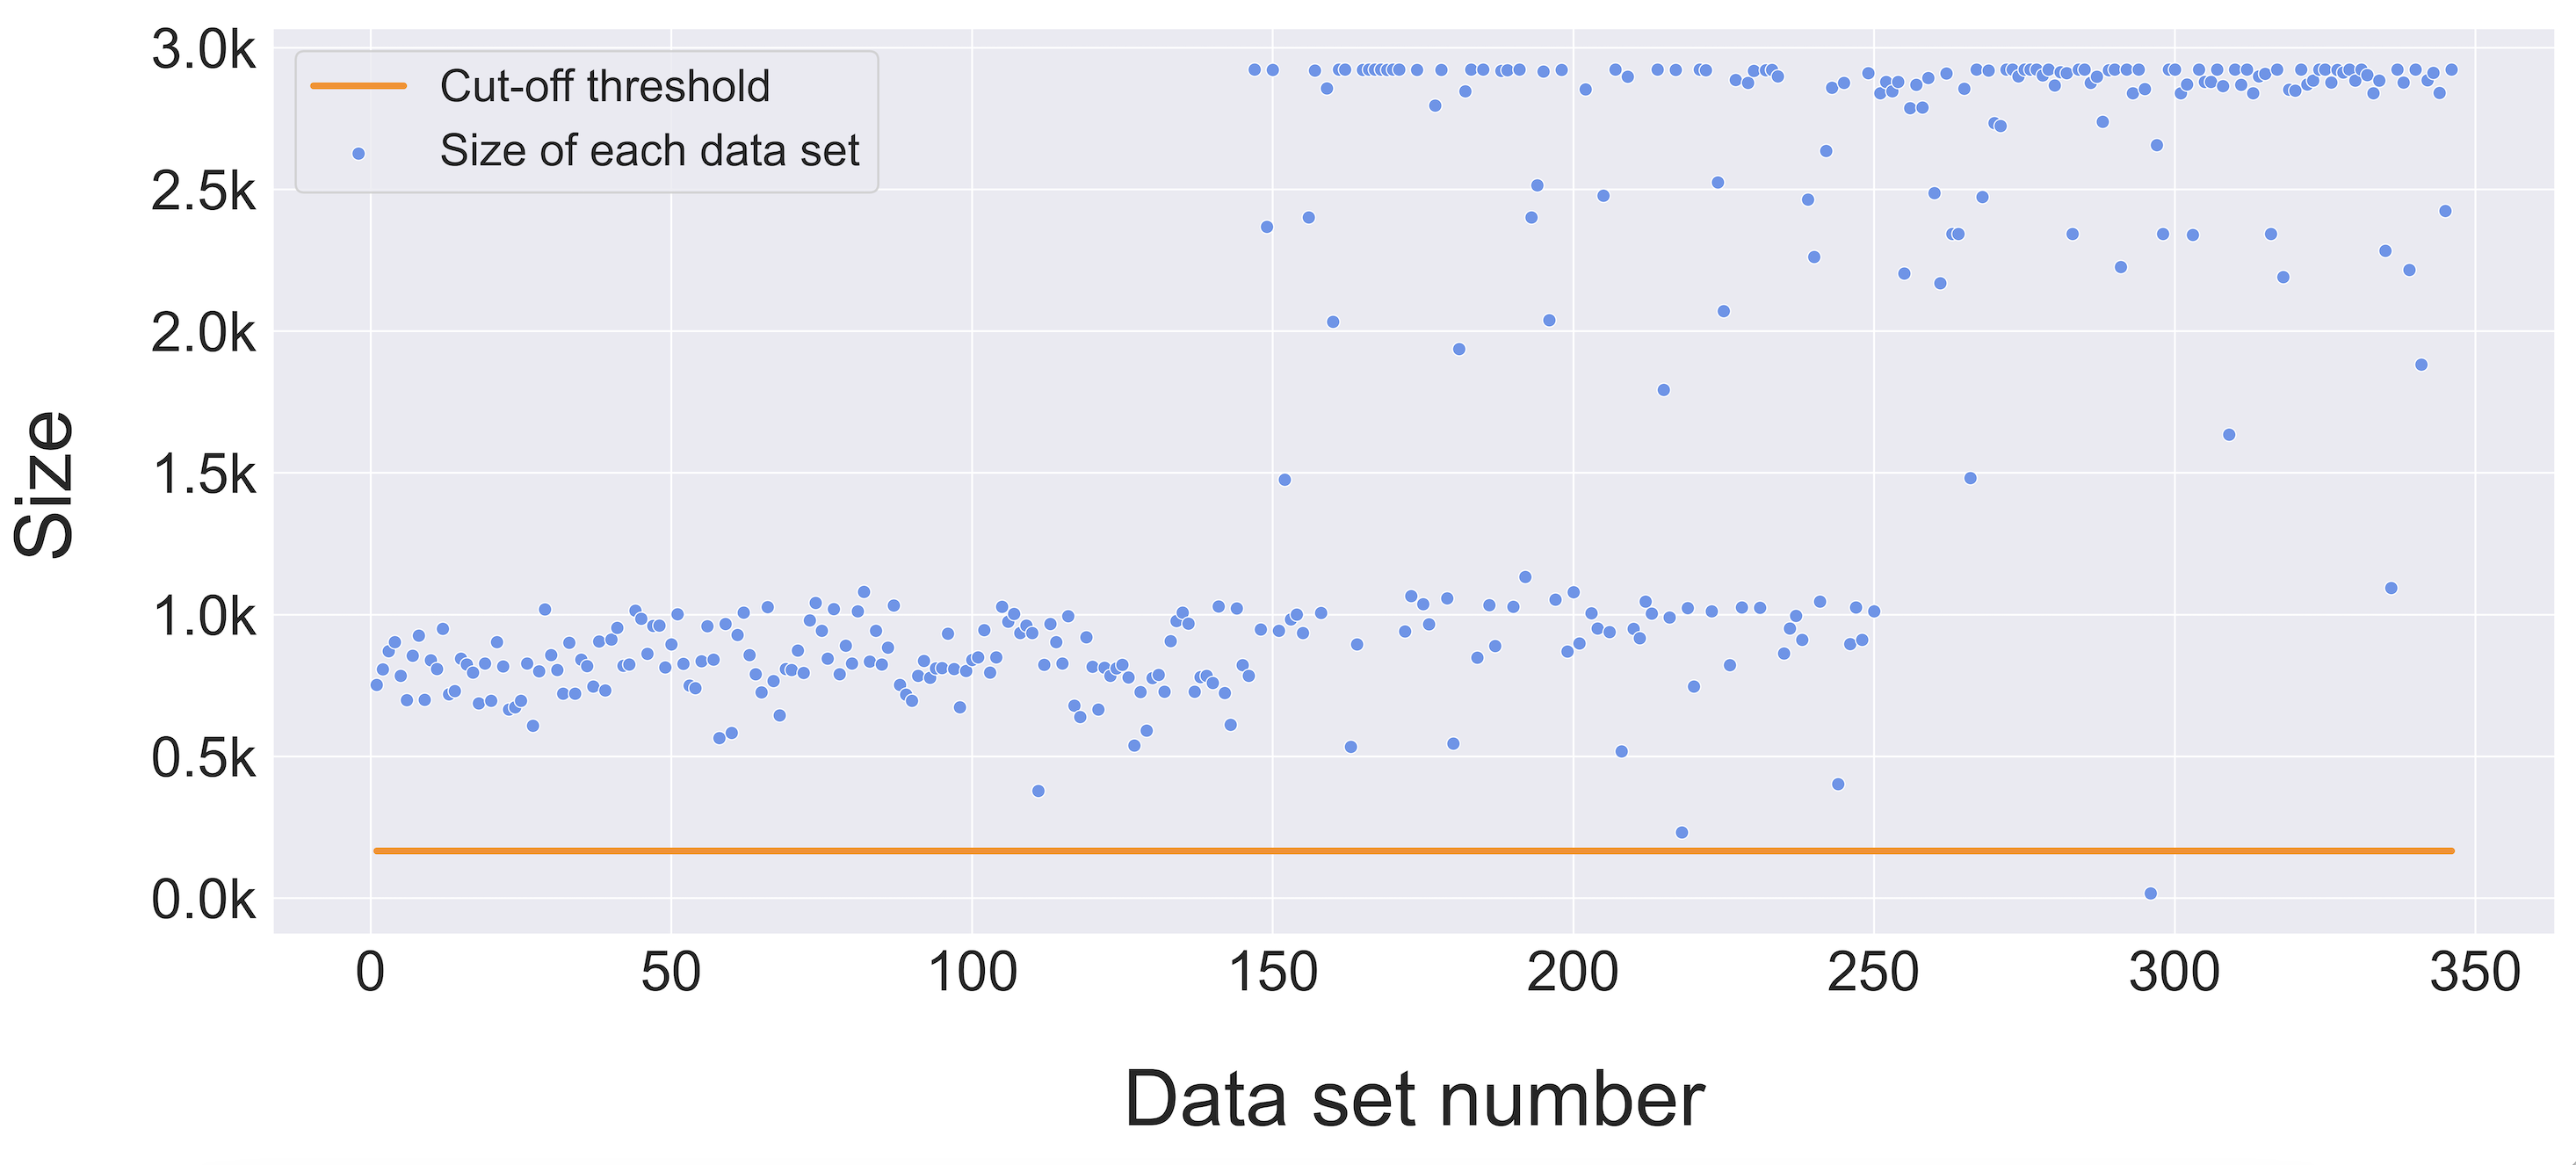
\includegraphics[width=1\textwidth]{Figures/dataset_Y.png}}
  \caption[Data set sizes]{The figures show the data set sizes of X and Y and the proposed cut-off threshold at 10 $\%$ of the mean set size.}
\end{figure}

\fi

%%%%%%%%%%%%%%%%%%%%%%%%%%%%%%%%%%%%%%%%%%%%%%%%%%%%%%%%
